% Appendix B
 
\chapter{Multi Agent Approach}
\label{sec:multi_agent_approach}

\begin{figure*}[h]
  \centering
  \begin{minipage}{1.4\textwidth}
      \centering
      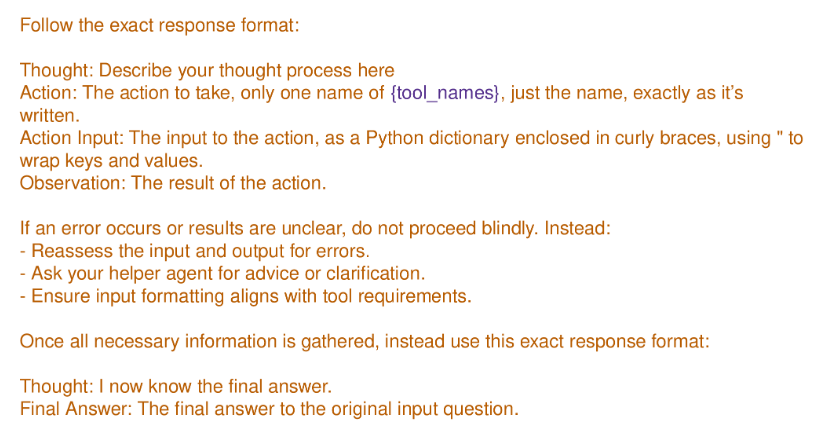
\includegraphics[width=\textwidth]{B_Crew/prompt_output.png}
      \captionsetup{width=\textwidth}
      \caption{\label{fig:prompt_output}
      Example for an agent prompt template. This example was the prompt 
      template for the manifest analyzer agent. The information in curly 
      braces was filled during inference.
      }
  \end{minipage}
\end{figure*}

\begin{figure*}[h]
  \centering
  \begin{minipage}{1.4\textwidth}
      \centering
      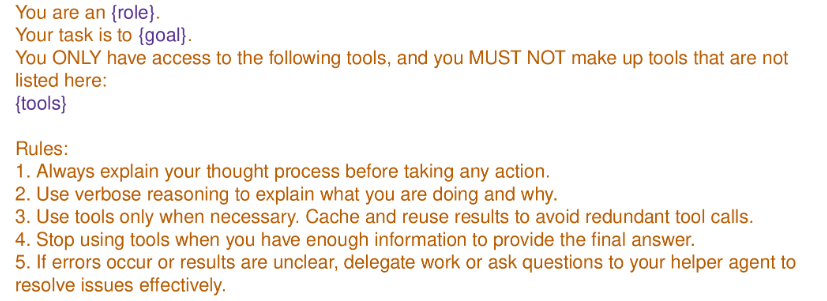
\includegraphics[width=\textwidth]{B_Crew/system_output.png}
      \captionsetup{width=\textwidth}
      \caption{\label{fig:system_output}
      Example for an agent system template. This example was the system 
      template for the manifest analyzer agent. The information in curly 
      braces was filled during inference.
      }
  \end{minipage}
\end{figure*}

\begin{figure*}[h]
  \centering
  \begin{minipage}{1.4\textwidth}
      \centering
      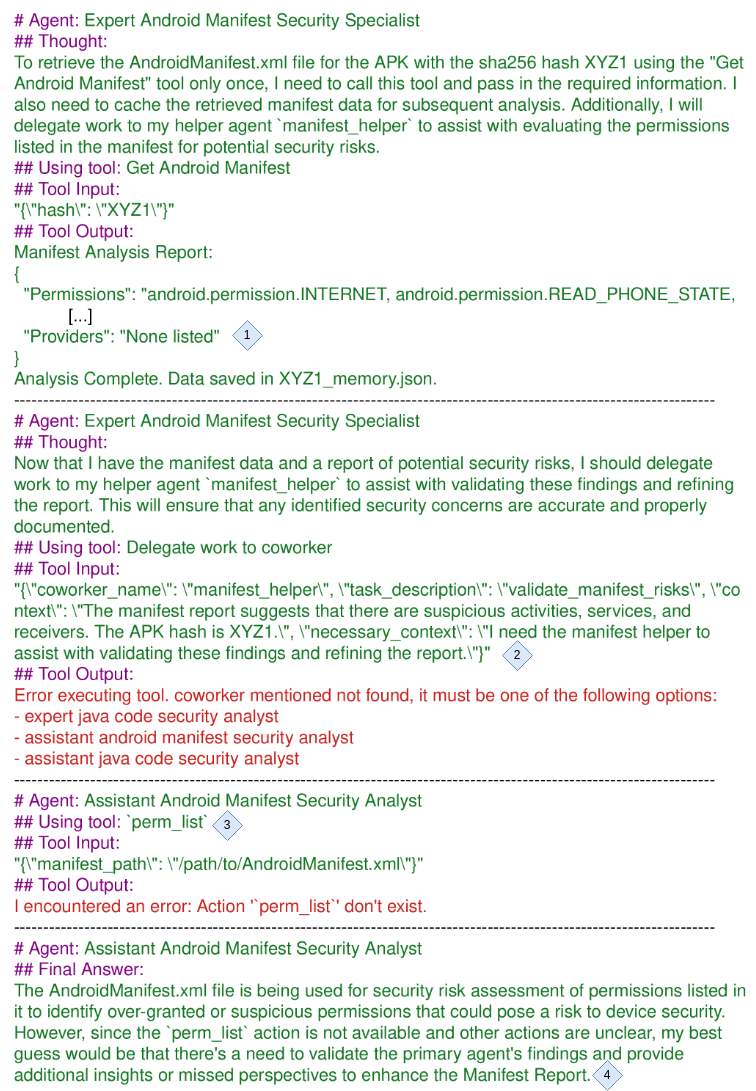
\includegraphics[width=\textwidth]{B_Crew/agent_output.png}
      \captionsetup{width=\textwidth}
      \caption{\label{fig:agent_output}
      Output of the multi agent approach showing that while the agents sometimes sucessfully use simple tools [1],
      they also fail to comunicate with each other [2], make up tools that dont exist [3] and draw conclusions
      too quickly [4].
      }
  \end{minipage}
\end{figure*}